\chapter{数值实验}
\section{数值实验准备}
为了验证算法对目标状态定位跟踪的准确性,本章对算法进行了一些必要的数值实验.为了便于比较算法的定位效果,在此给出目标在 $iT$ 时刻的位置坐标的相对误差 $MSE1$:
\begin{equation}
	MSE1 = \frac{\sqrt{(x_i-\hat{x}_i)^2 + (y_i -\hat{y}_i)^2 +(z_i -\hat{z}_i)^2}}{\sqrt{(x_i-B_{ix})^2 +(y_i - B_{iy})^2 + (z_i - B_{iz})^2}}
\end{equation}
目标速度的相对误差为 $MSE2$:
\begin{equation}
	MSE2 = \frac{\sqrt{(v_x-\hat{v}_{ix})^2 + (v_y-\hat{v}_{iy})^2 + (v_z-\hat{v}_{iz})^2 }}{\sqrt{v_x^2 +v_y^2 + v_z^2}}
\end{equation}
其中 $\bm{x}_i = (x_i,y_i,z_i,v_x,v_y,v_z)^T$ 为目标在 $iT$ 时刻的真实状态矢量,$\hat{\bm{x}}_i = (\hat{x}_i,\hat{y}_i,\hat{z}_i,\hat{v}_{ix},\hat{v}_{iy},\hat{v}_{iz})^T$ 为目标在 $iT$ 时刻的估计状态矢量.
\section{初步实验}
让观测站在 $X$ 轴上运动,观测站的加速度矢量为
 $\bm{a} = [0.01,0,0]^T$,初始速度为 $\bm{v}_B = [0,0,0]^T$,初始位置为 $B_0 = (5km,0,0)^T$,在 $(x_0,y_0,z_0) \in [500km,1000km]\times[500km,1000km]\times[500km,1000km]$,$(v_x,v_y,v_z) \in [0,0.5km/s]\times[0,0.5km/s]\times[0,0.5km/s]$的范围随机选取 $(x_0,y_0,z_0,v_x,v_y,v_z)$ 作为目标的初始状态矢量,且目标做匀速运动.在60s的时间内,观测站从0时刻开始每隔 $T=0.1s$ 对目标的角度信息进行一次观测,最后利用60s内所观测的数据对目标的初始状态求解.做100次Monte Carlo实验,并取 $\sigma = 0.00005rad$,做出各算法求解的误差图如下:

\begin{figure}[htbp]
	\vspace{13pt}
	\centering
	\subfigure[距离相对误差图]{
	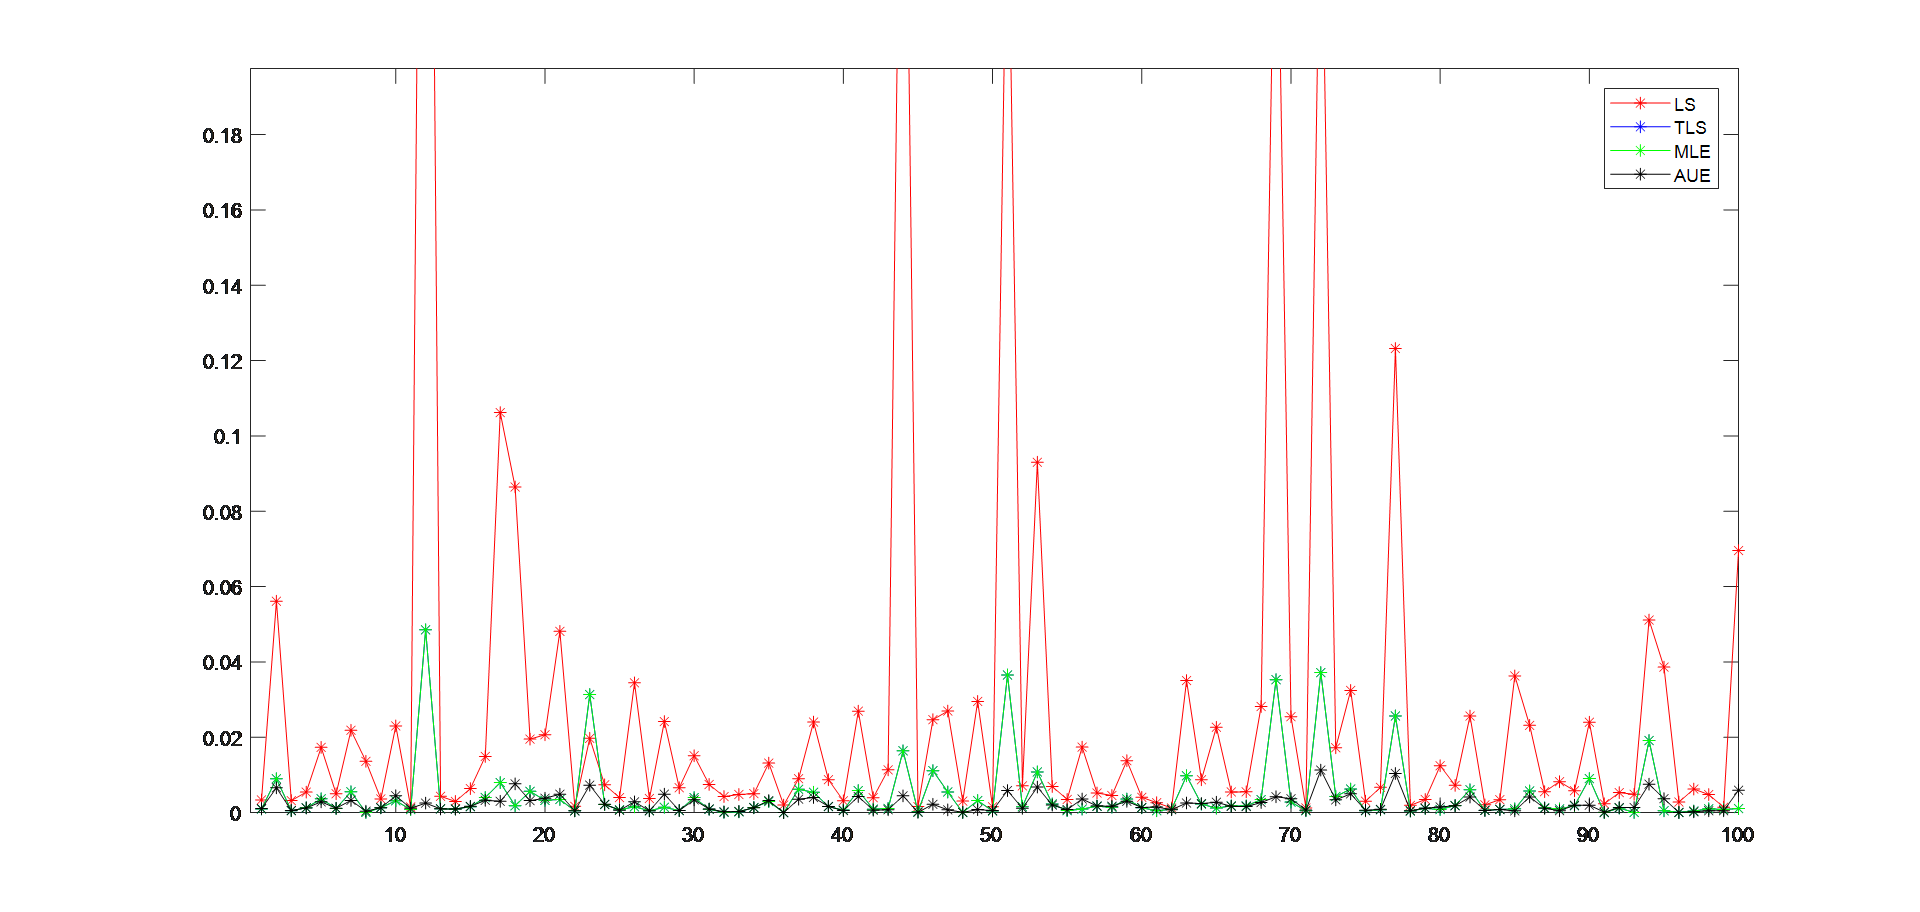
\includegraphics[width=\linewidth]{images/100MonteCarlo.png}	
} 

	\subfigure[速度相对误差图]{
	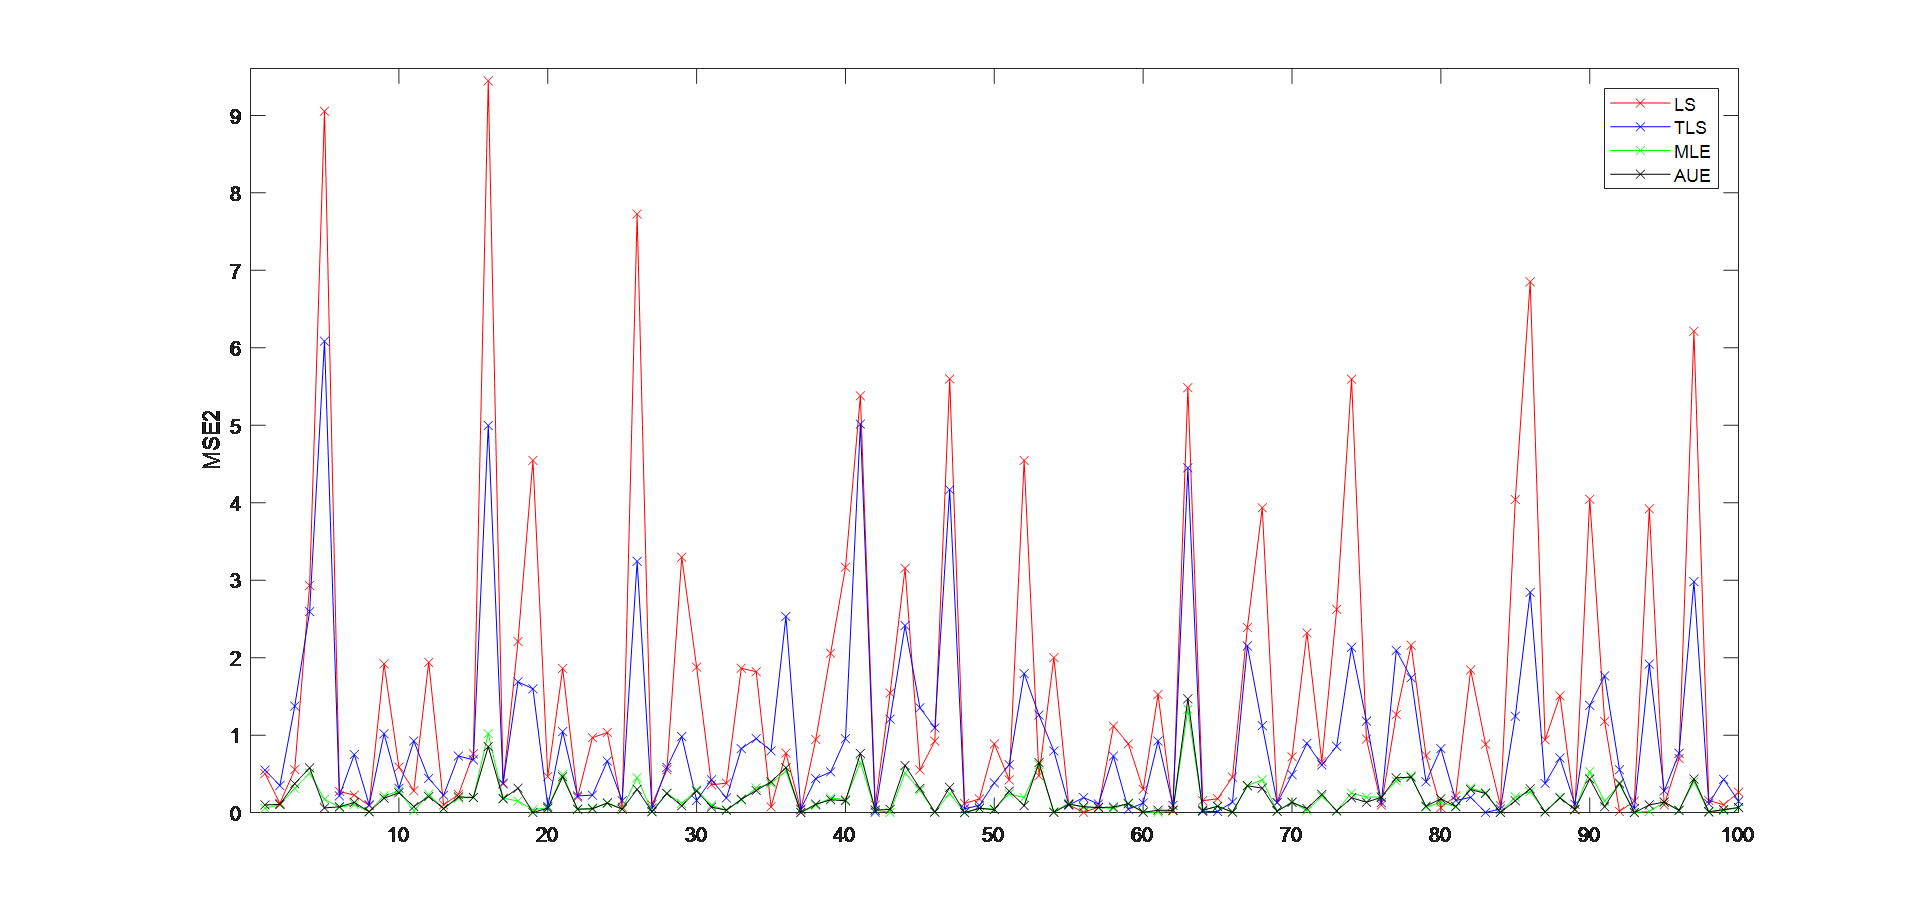
\includegraphics[width=\linewidth]{images/100MC_MSE2.png}	
}
	\caption{100次Monte Carlo实验各算法误差分析}
\end{figure}

\newpage

根据上图,在100次Monte Carlo实验中,对目标的初始状态 $\bm{X}_0$求解结果的相对误差进行比较.从距离相对误差图来看,AUE算法和MLE算法的结果相对较好,且受噪声的影响相对于其它两种算法较小,TLS算法相对于OLS算法表现的较好,但是受噪声的影响较大,不稳定.OLS算法表现结果相对较差,受噪声影响最大.从速度相对误差图来看,AUE算法和MLE算法的结果相对较好,误差范围大致在 $0 \sim 0.5$ 之间,而TLS算法和OLS算法得到的结果并不稳定,受噪声影响较大.

在不改变观测站运动状态的情况下,取 $(50km,60km,70km,0.5km/s,0.4km/s$, $ 0.2km/s)$ 做为目标的初始状态矢量,取 $\sigma=0.00005$,根据 $iT$ 时刻($T=0.1s$)前的观测数据来计算目标在 $iT$ 时刻的状态矢量 $\bm{X}_i$,得到误差图如下:
\begin{figure}[htbp]
	\centering
	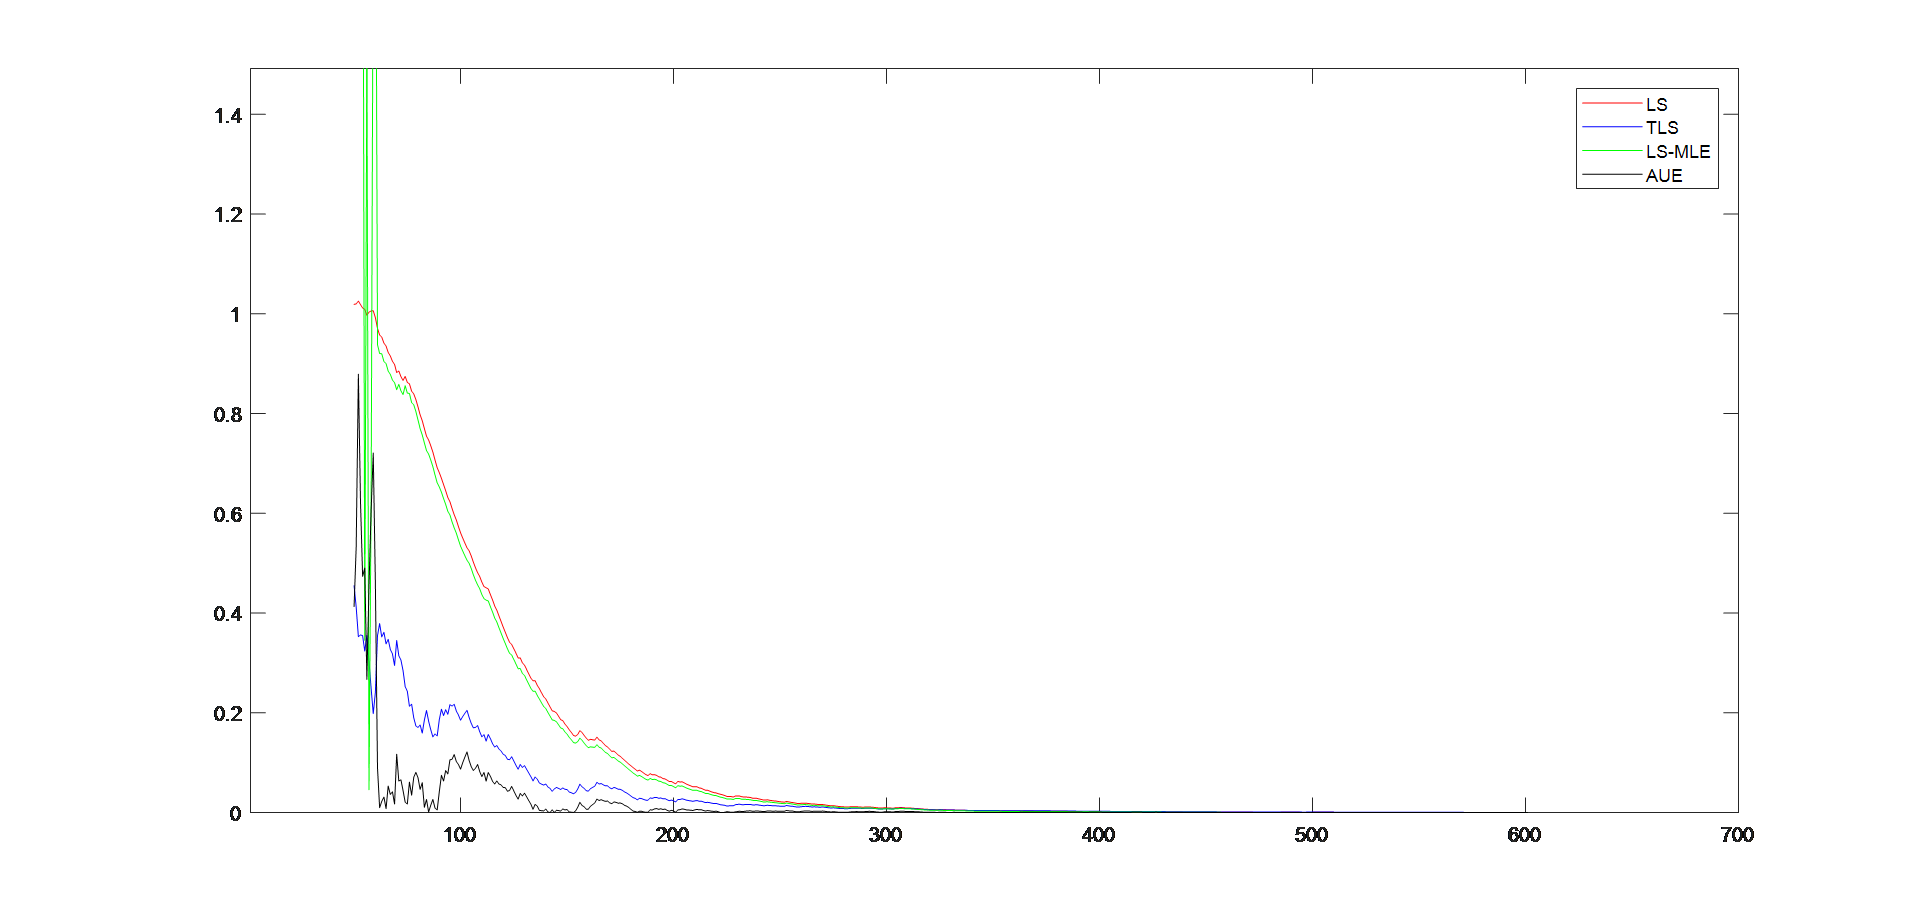
\includegraphics[width=\linewidth]{images/singleline.png}
	\caption{距离相对误差图}
\end{figure}

根据距离相对误差图分析,随着观测时间的增加各个算法求解的位置相对误差在不断减小,在15s时初步达到较为精确的定位.可以判断随着测量信息量的增多,算法对目标的运动轨迹判断变得更为准确,降低了噪声的影响,使定位更加准确.其中AUE算法和TLS算法求解的结果较好,最先得到较为准确的结果.

根据图4-3的速度相对误差图可知,随着观测时间的增加各个算法求解的速度相对误差在不断减少,但是求解得到的误差仍比较大,在15s时初步得到较为准确的结果.其中AUE算法和TLS算法最先得到较为准确的结果.
\newpage
\begin{figure}[htbp]
	\vspace{6pt}
	\centering
	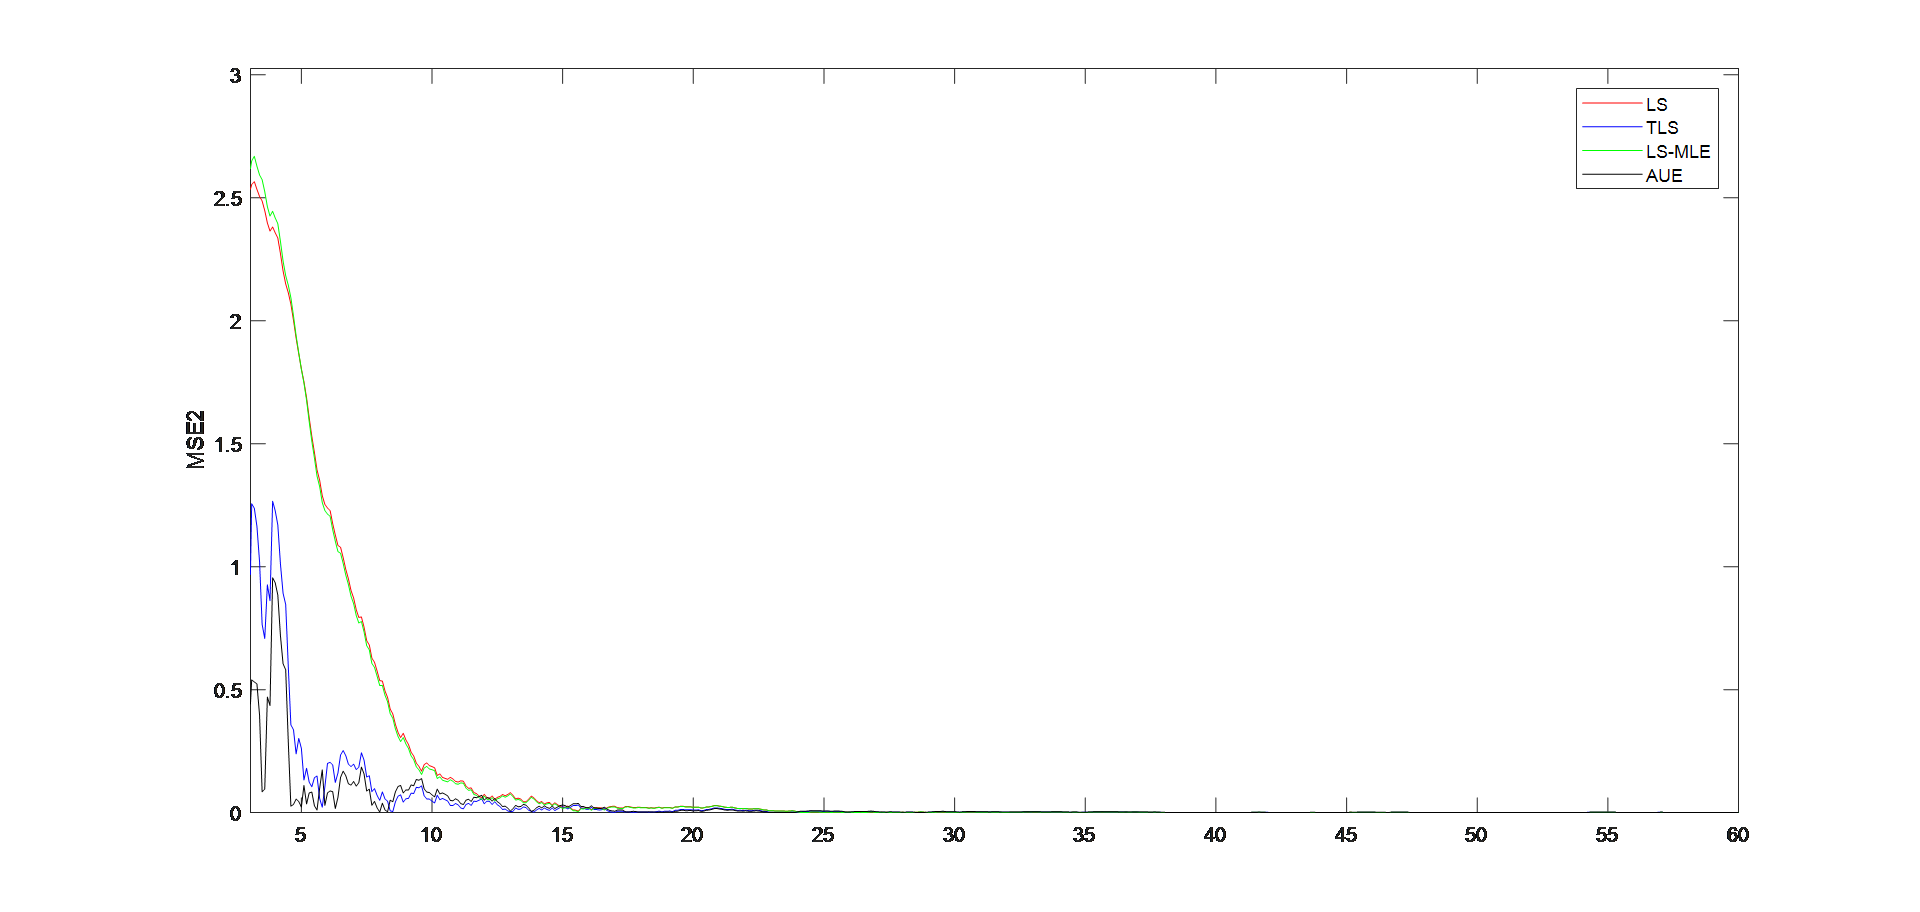
\includegraphics[width=\linewidth]{images/line_v.png}
	\caption{速度相对误差图}
\end{figure}

为了更好的分析求解情况,取出15s之后的误差结果图,判断各个定位算法的求解精度,误差结果图如图4-4和图4-5所示.

\begin{figure}[h]
	\centering
	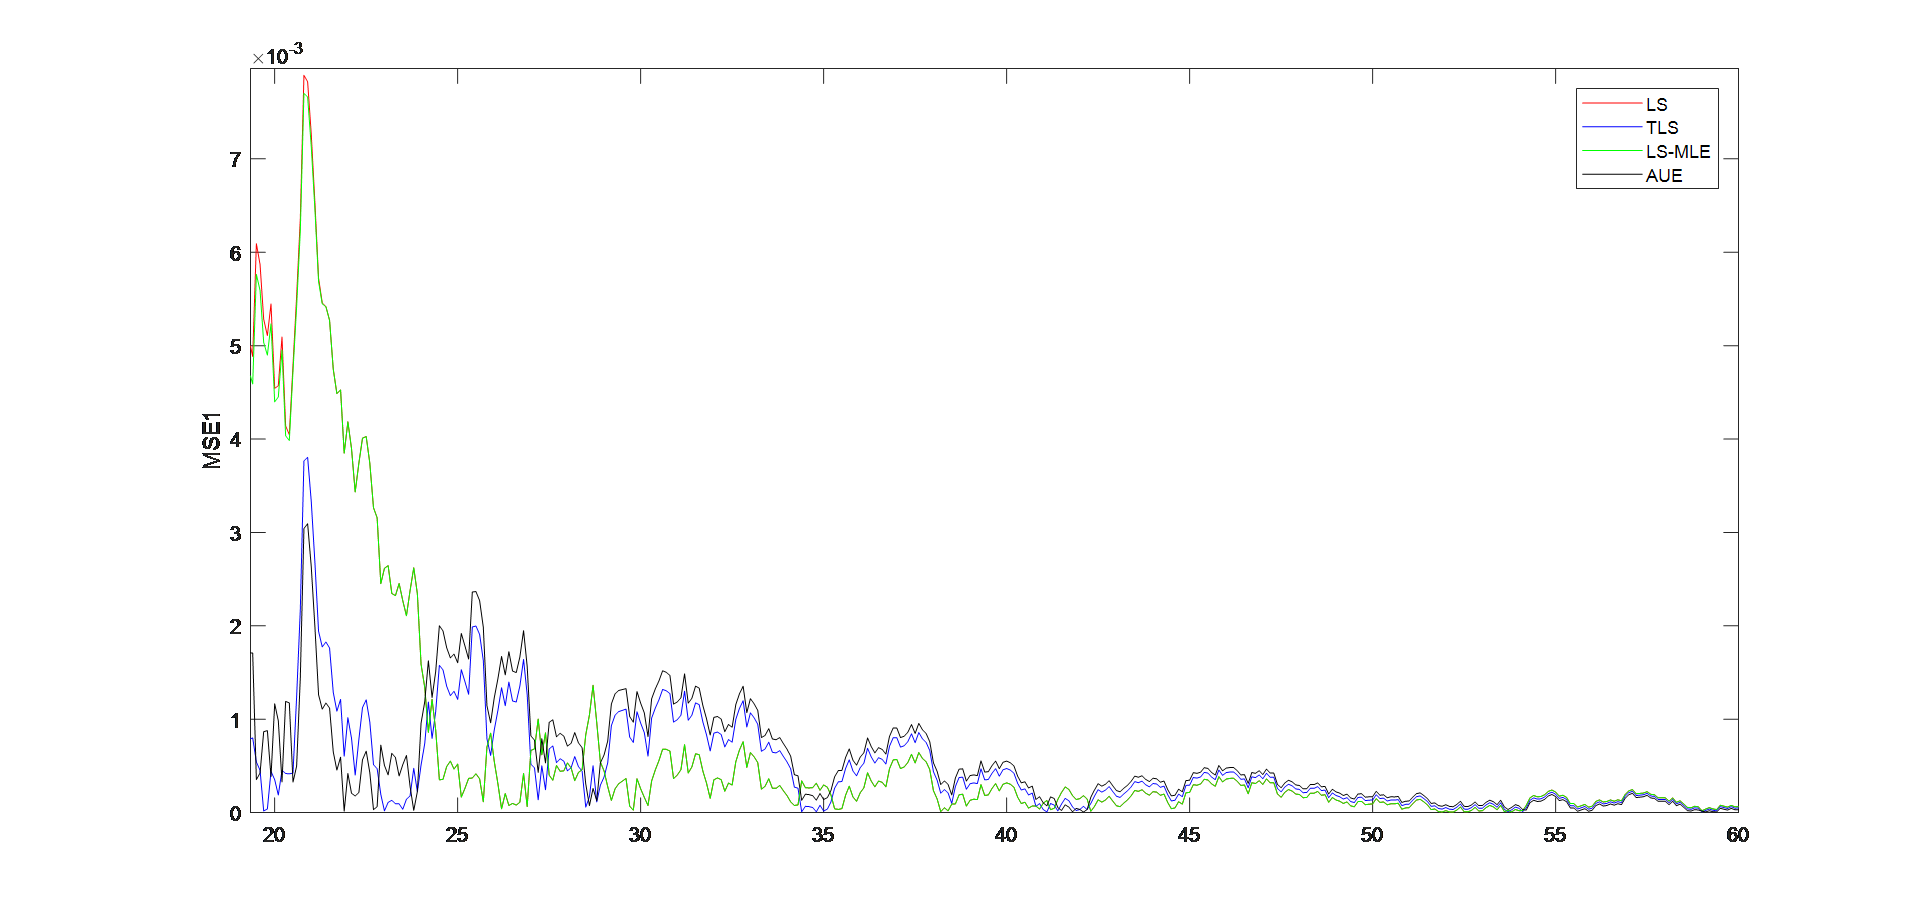
\includegraphics[width=\linewidth]{images/zoomsingleline.png}
	\caption{15s后的距离相对误差图}
\end{figure}
据图4-4和图4-5可知,在当前实验条件下,在15s之后四种算法求解得出的距离误差和速度误差都比较小,而且在40s之后,四种算法求解得到的误差没有明显区别,基本一致.
\newpage
\begin{figure}[htbp]
	\vspace{13pt}
	\centering
	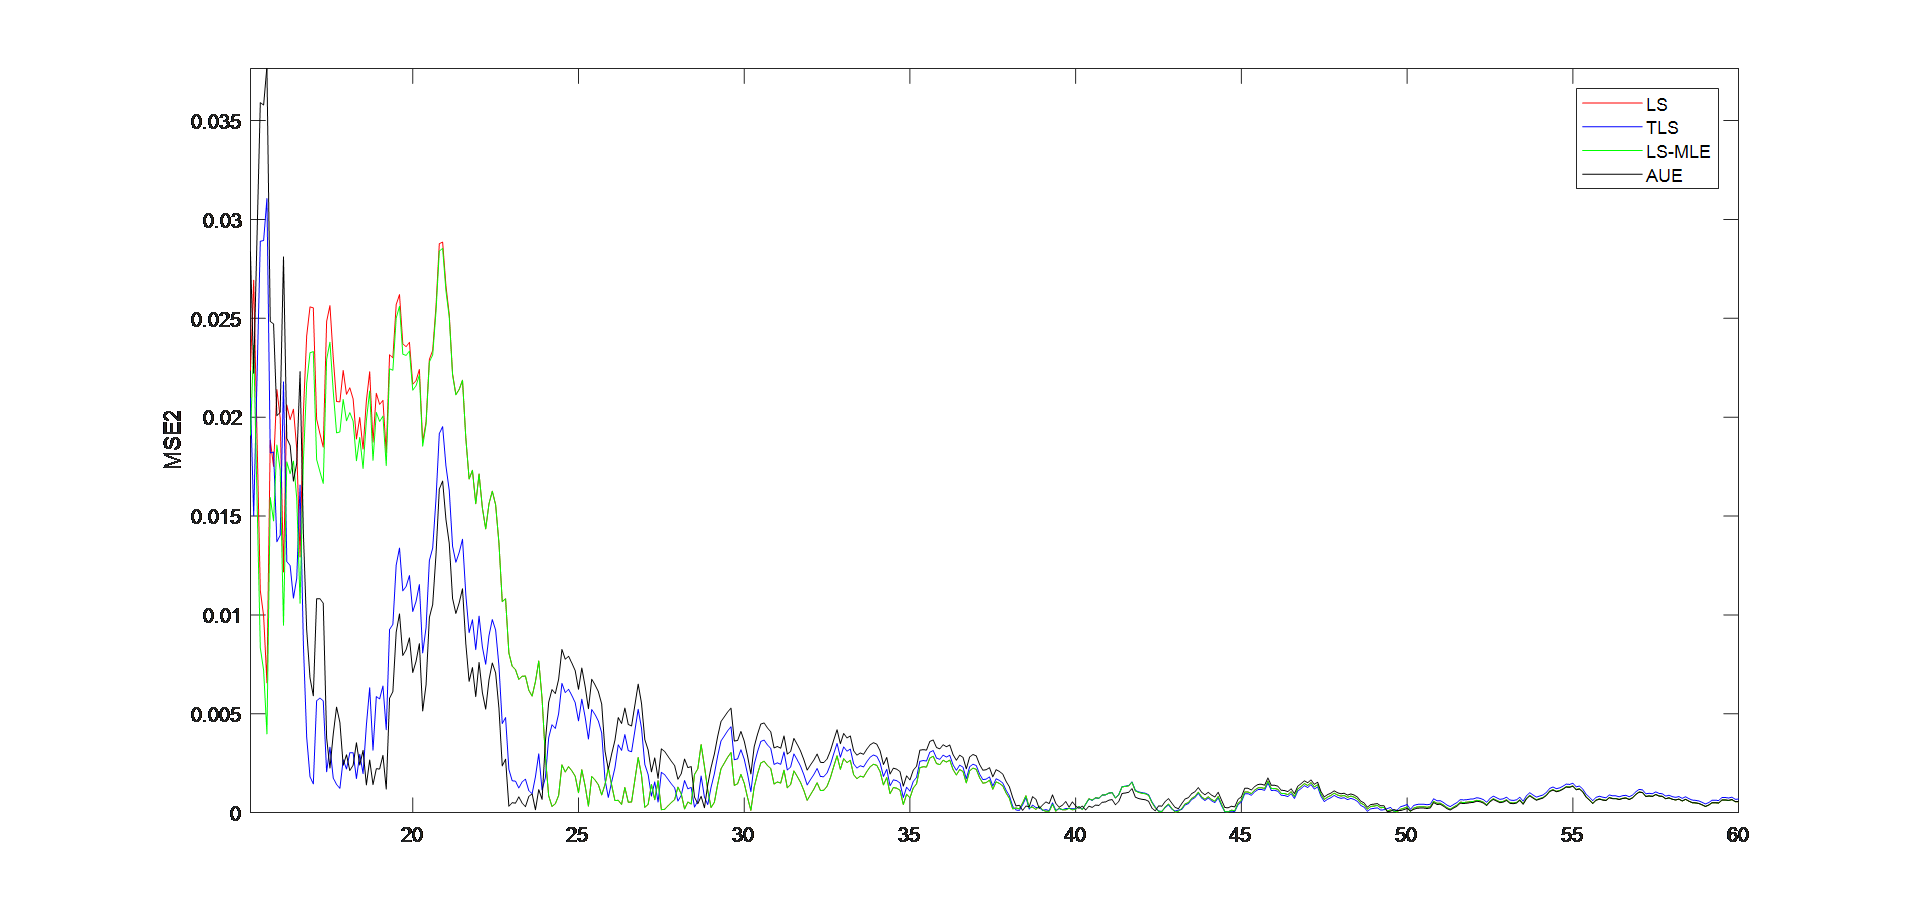
\includegraphics[width=\linewidth]{images/line_vzoom.png}
	\caption{15s后的速度相对误差图}
\end{figure}

根据以上初步实验分析可知,AUE算法对目标的轨迹求解较好,可以在相对较少测量信息的条件下得到较为精确的值.OLS算法和TLS算法对目标轨迹求解结果不稳定,容易出现较差求解结果.MLE算法在信息量足够的情况下也能得到较好的求解结果,但在信息量较少的时候求解的较差,且MLE算法的求解结果取决于初值的选取,迭代过程中产生的计算量相对较大,而且可能会出现不收敛的情况,因此在接下来的实验中暂时不考虑MLE算法.
\section{观测站与目标的距离对算法结果的影响}
为了研究观测站与目标的距离对算法的影响,考虑如下实验条件:

观测站在 $X$ 轴上运动,其加速度矢量为 $\bm{a}=(0.01,0,0)$,初始速度为 $\bm{v}_B = (0,0,0)$,目标的运动速度为 $\bm{v} = (0.3km/s,0.4km/s,0.5km/s)$.在60s的时间内,观测站从0时刻开始每隔0.1s对目标的角度信息进行一次测量,然后利用60s内观测的信息对目标的初始状态求解.在该条件下进行200次实验,其中目标的初始速度为 $\bm{v}=(0.3km/s,0.4km/s,0.5km/s)$,第一次实验时目标的初始位置坐标为 $(50km,50km,50km)$,之后每次实验目标的初始位置坐标在上一次的基础上增加 $(5km,6km,6km)$,假设每次实验测量角度的噪声相同,且取$\sigma=0.00005rad$,得到算法的求解误差图如下:
\newpage
\begin{figure}[htbp]
	\vspace{13pt}
	\centering
	\subfigure[距离相对误差图]{
	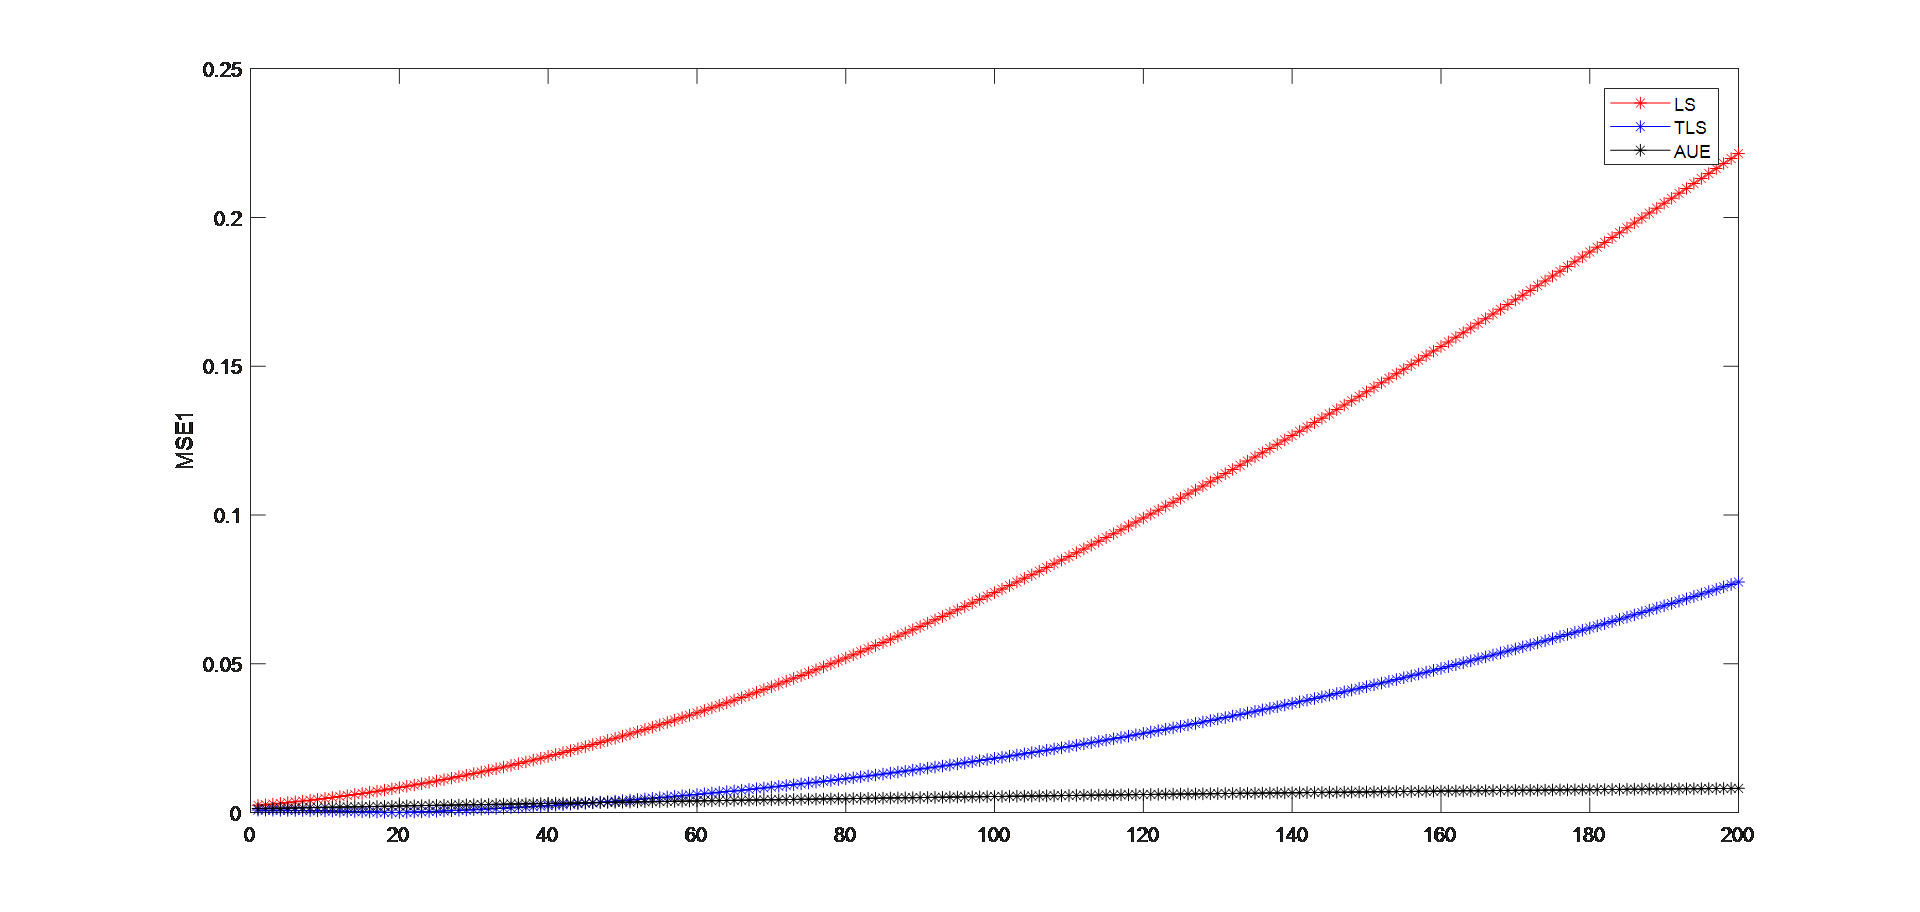
\includegraphics[width=\linewidth]{images/distence_MSE1.png}	
}

	\subfigure[速度相对误差图]{
	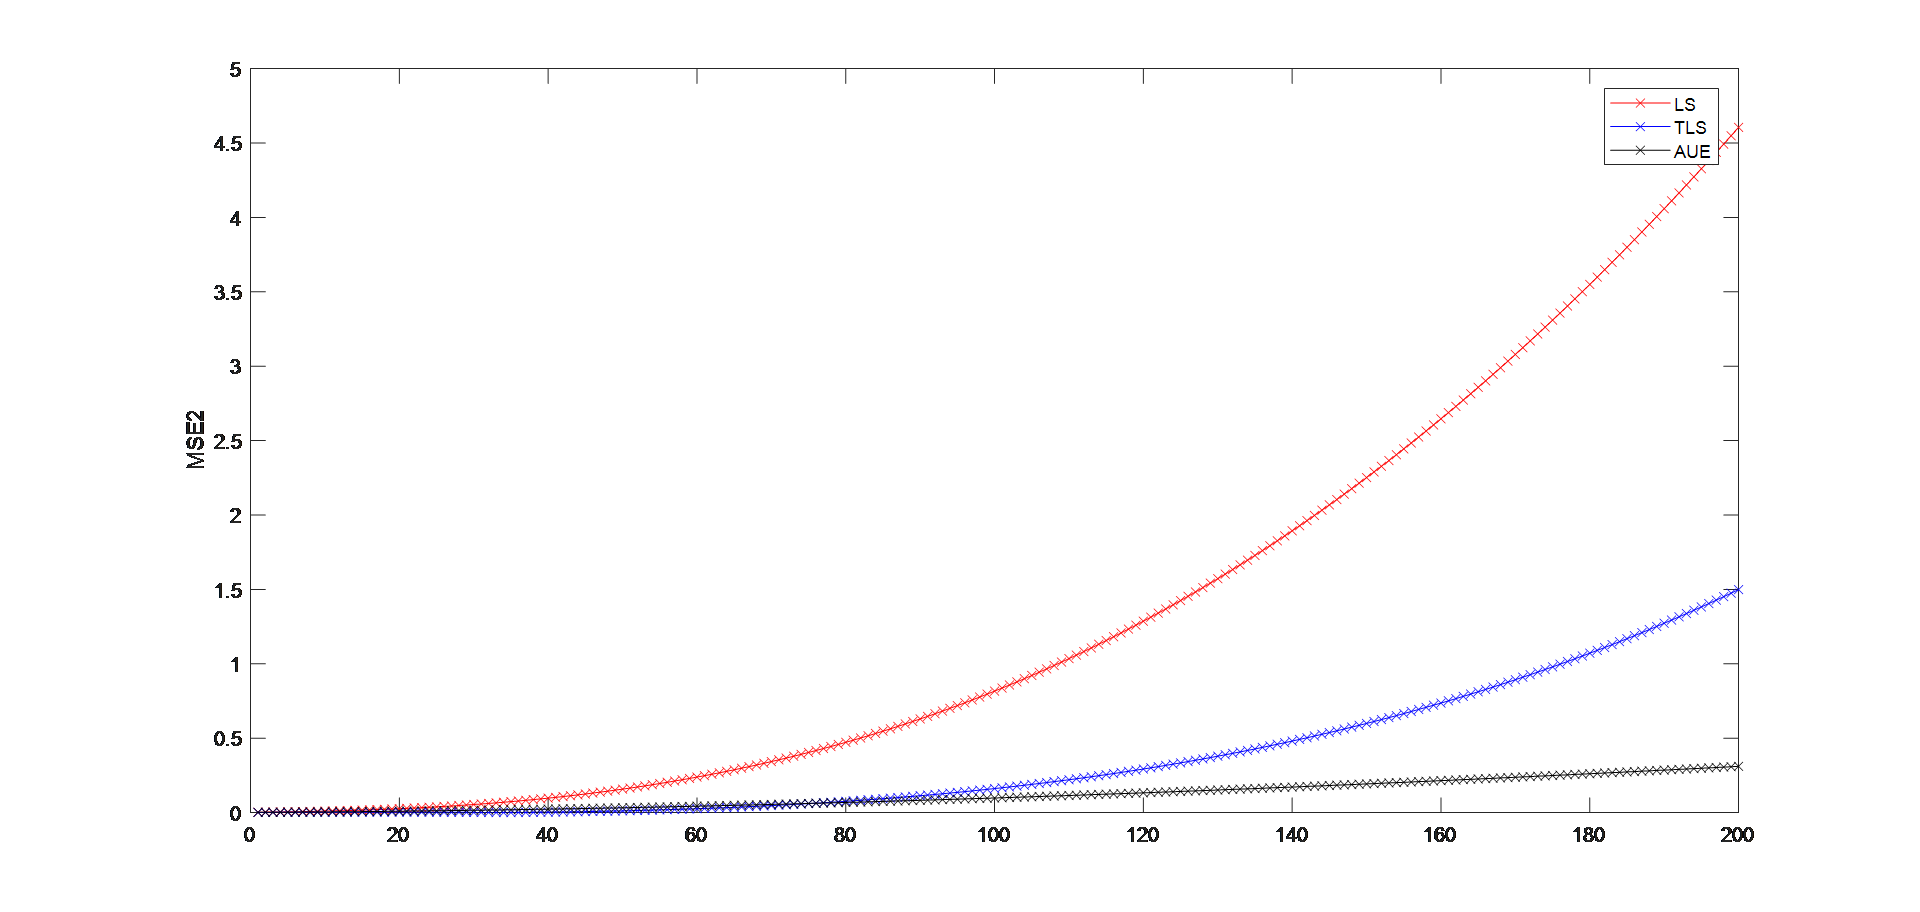
\includegraphics[width=\linewidth]{images/distence_MSE2.png}	
}
	\caption{随距离增加的误差图}
\end{figure}

从图中可以发现,在相同噪声条件下,三种算法求解得到的目标初始状态的相对误差和目标距离观测站的距离呈现一种正相关的关系.其中,OLS算法求解得到的相对误差增加最明显,TLS算法求解得到的相对误差大概在目标初始位置距离观测站约500km时才开始缓慢增加,AUE算法求解得到的相对误差随距离的增加相对于OLS算法和TLS算法增加的并不明显.出现该结果的原因可能是,在目标和观测站距离较近时,观测站每0.1s测得的角度信息的差值较大,受噪声的影响相对较小,因此计算得到的相对误差较小.但是当目标和观测站之间的距离不断变大时,观测站测得的方位角及仰角的数据较为紧凑,差值较小,受噪声的影响较大,因此计算得到的相对误差变大.不过AUE算法做为一种无偏估计算法,受噪声影响程度比其它两种算法小.

三种算法对距离的求解估计精度较高,对速度的估计精度较低,这可能是由于观测角度存在噪声的影响使得测得的目标的运动方向在不断改变,从而使得算法对目标速度的估计存在较大的偏差.

\begin{figure}[htbp]
	\centering
	\subfigure[距离相对误差]{
	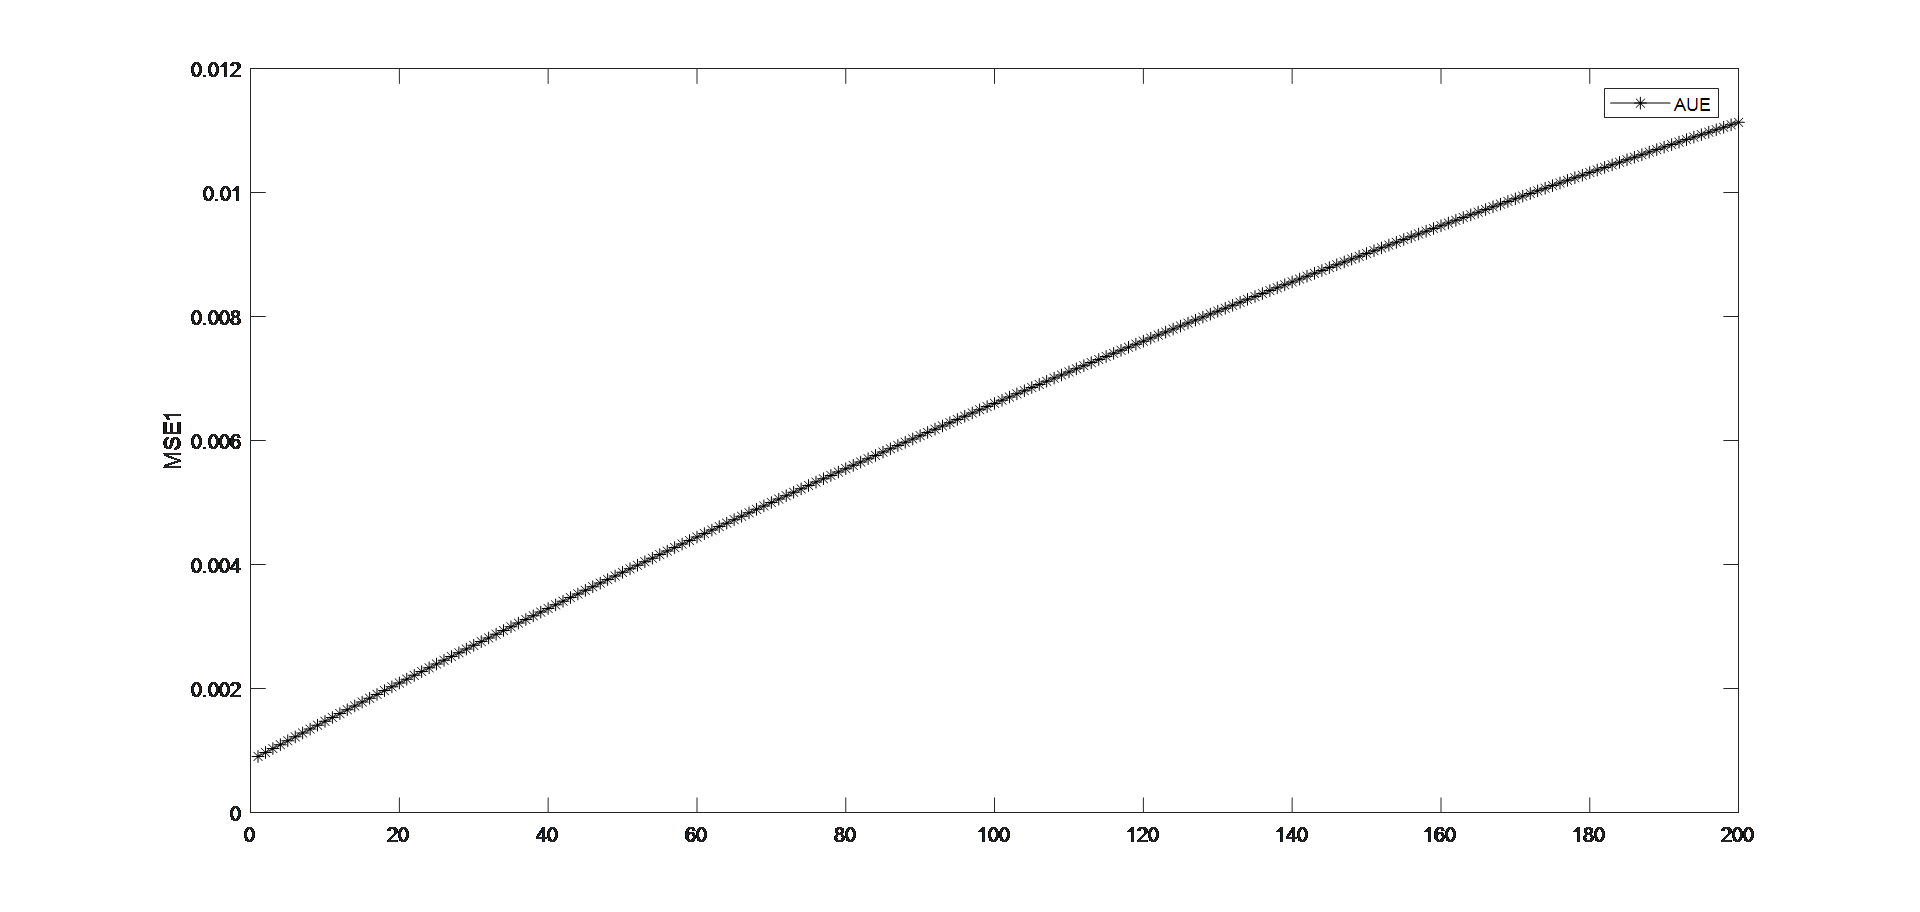
\includegraphics[width=\linewidth]{images/AUE_MSE1.png}
}
	
	\subfigure[速度相对误差]{
	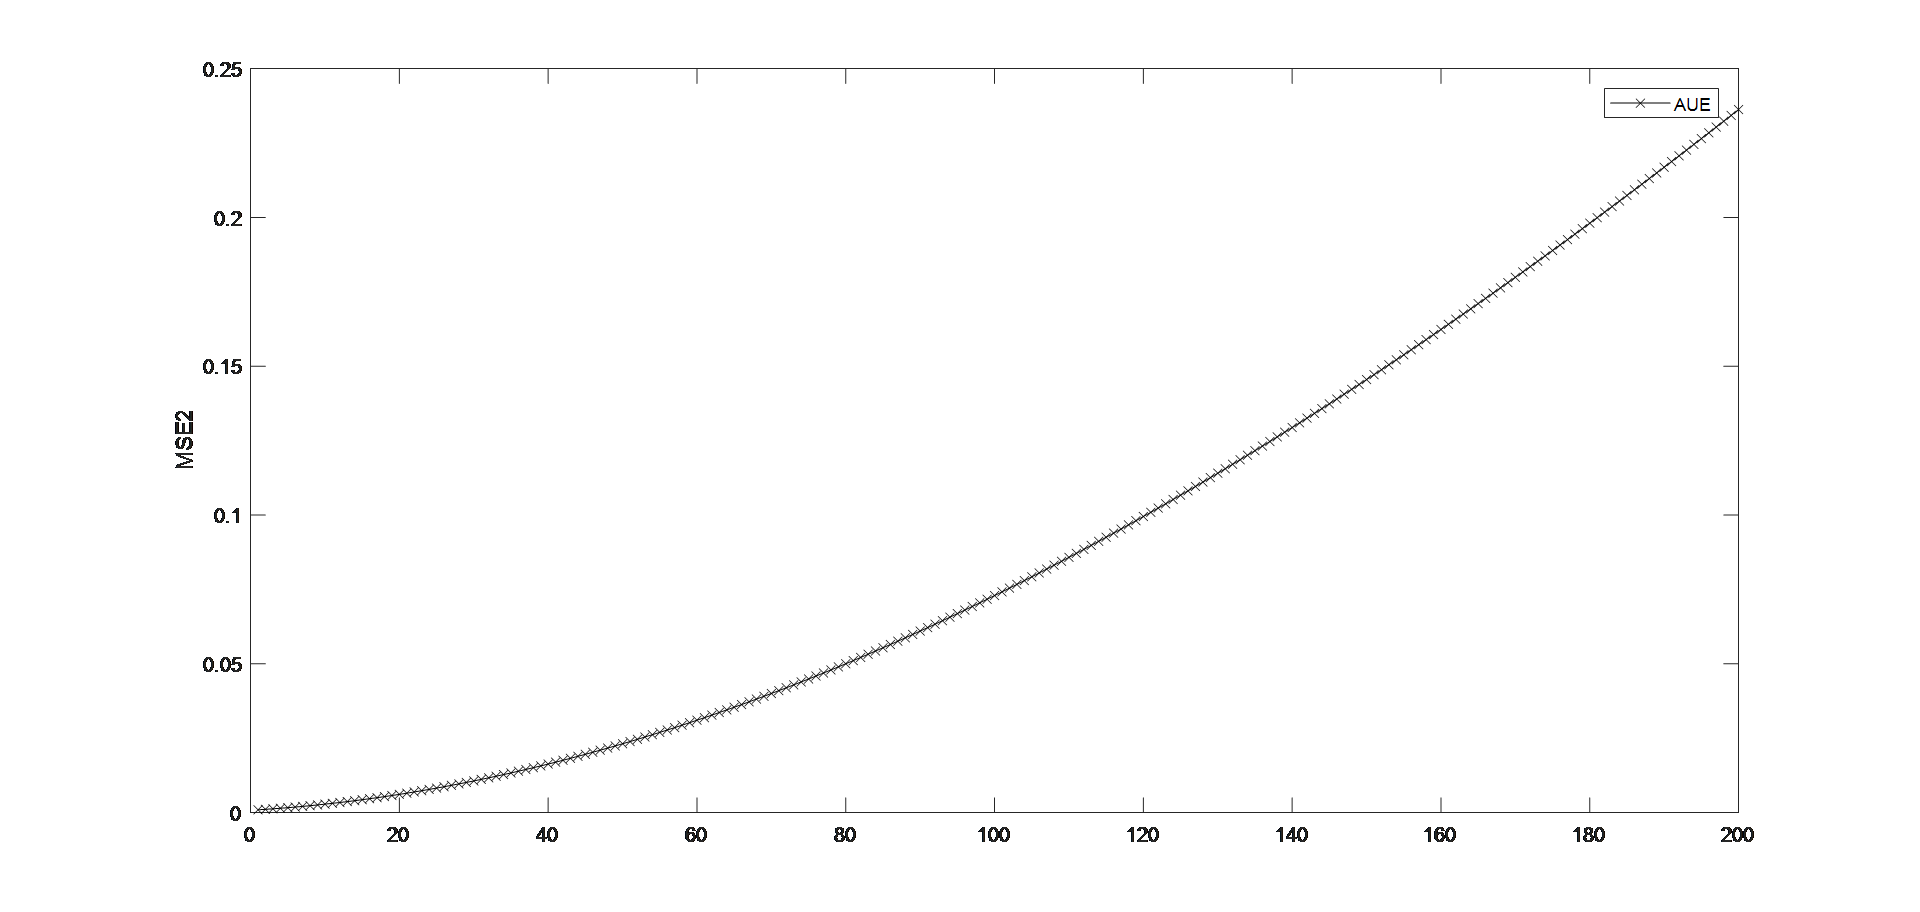
\includegraphics[width=\linewidth]{images/AUE_MSE2.png}	
}
	\caption{AUE算法随距离增加的计算误差图}
\end{figure}
图4-7将AUE算法随目标到观测站距离增加求解结果误差图单独画出,可以看到随距离增加算法的相对误差也在增加,且速度误差相对较大.
\section{方位角及仰角对算法结果的影响}
保持观测站运动状态不变,给定目标的初始位置为 $(500km,600km,400km)$,在第一次仿真实验中目标的速度为 $\bm{v}=(0.3km/s,0.2km/s,0.1km/s)$,取 $\sigma=0.00005rad$,每次使目标的初始速度增加 $(0,0,0.1km/s)$,在相同噪声条件下共进行20组仿真实验,得到求解结果的误差图:
\begin{figure}[htbp]
	\centering
	\subfigure[距离相对误差图]{
	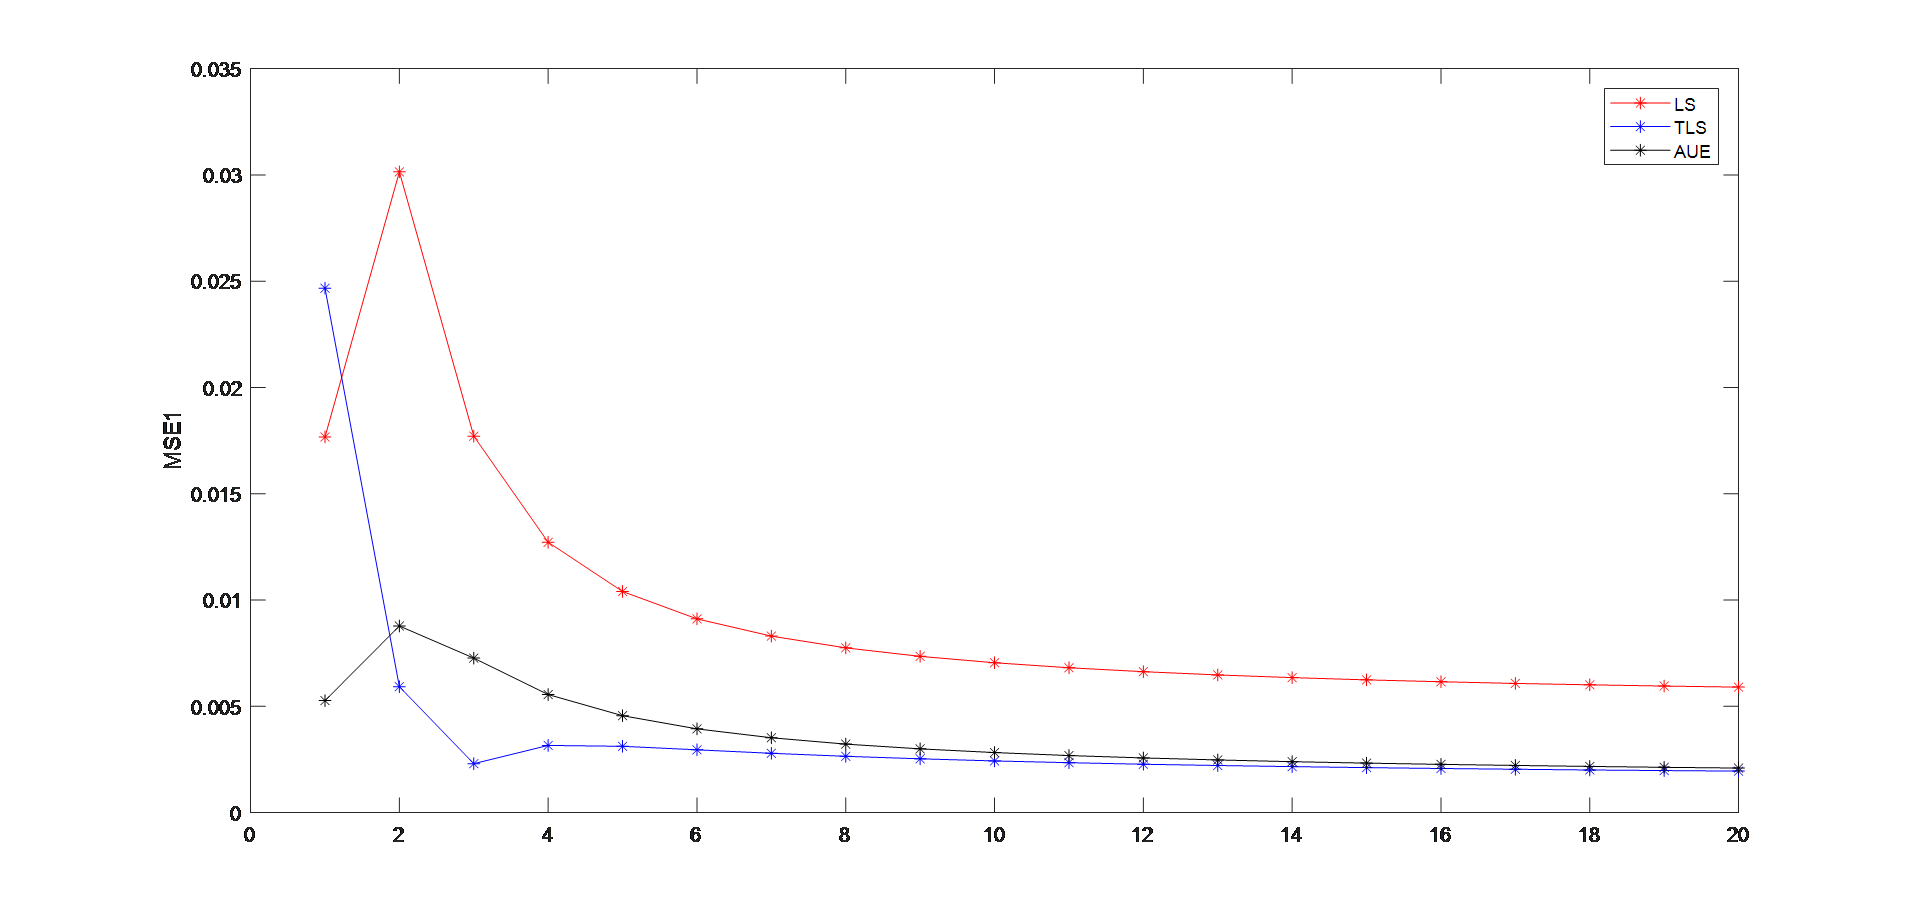
\includegraphics[width=0.93\linewidth]{images/elevation_MSE1.png}	
}

	\subfigure[速度相对误差图]{
	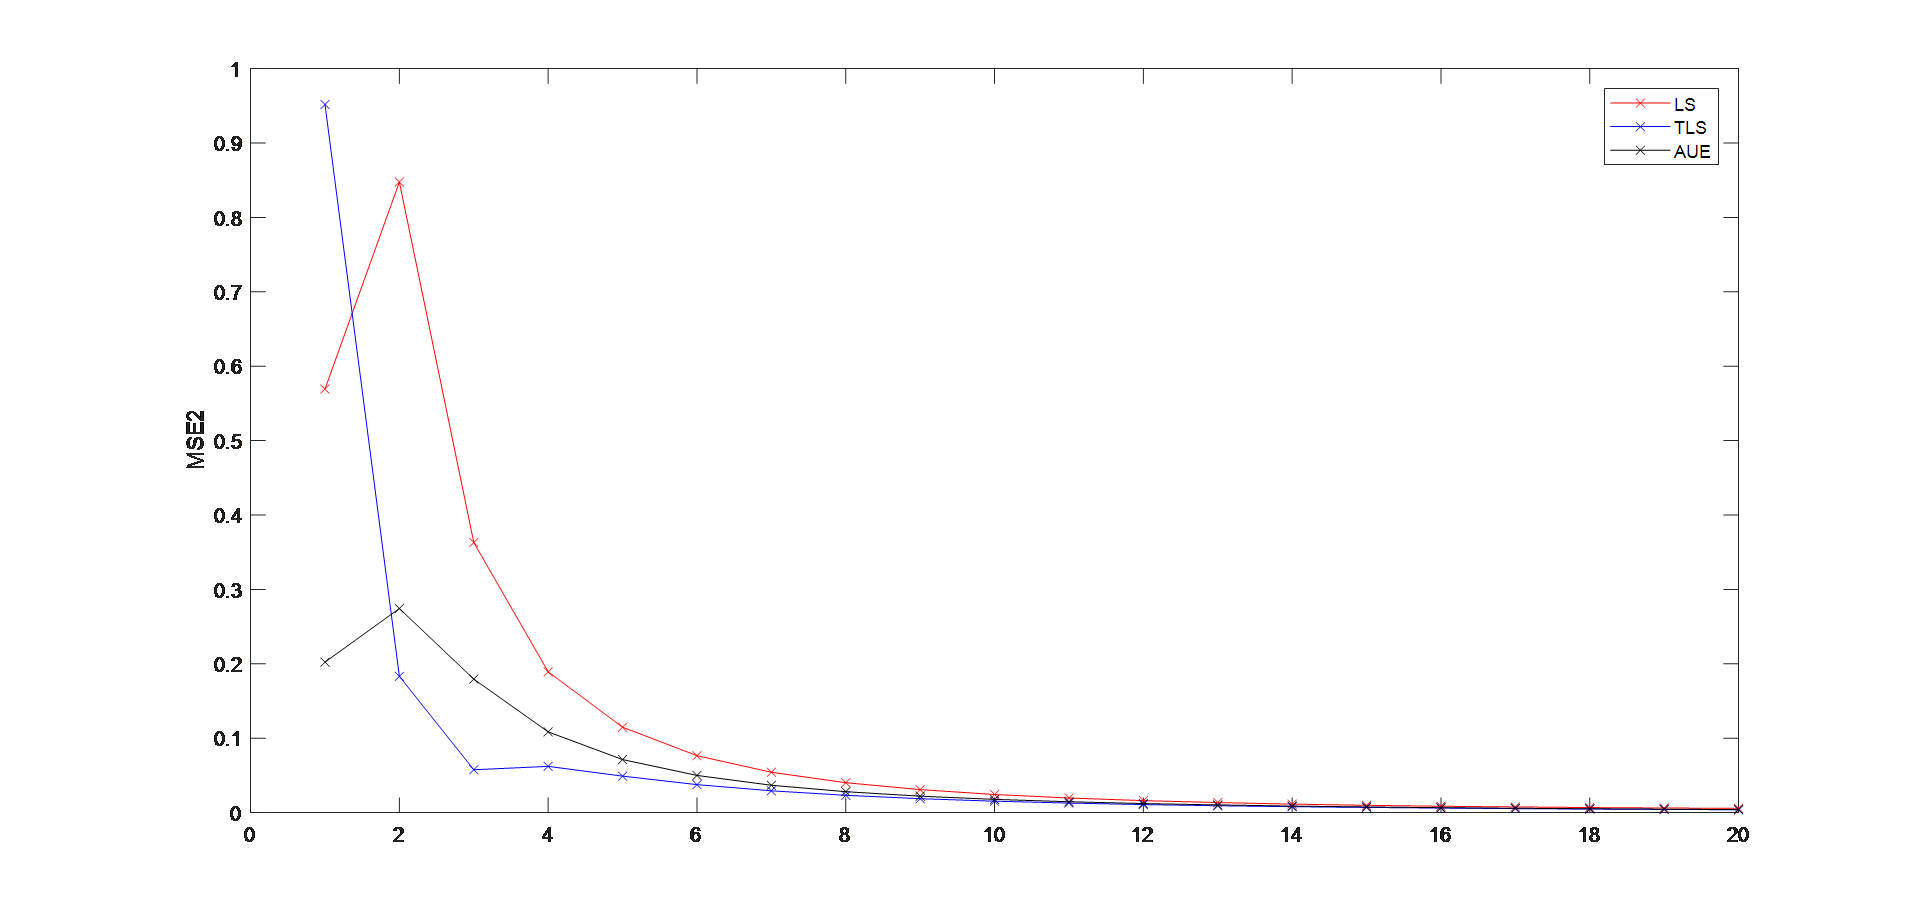
\includegraphics[width=0.93\linewidth]{images/elevation_MSE2.png}	
}
	\caption{仰角变化对结果的影响}
\end{figure}

在上述仿真实验条件中,改变第一次实验中目标的速度为 $\bm{v} = (0.1km/s,0.2km/s,0)$,速度每次增加 $(0.1km/s,0.2km/s,0)$,进行20组仿真实验,得到求解结果的误差图:
\begin{figure}[htbp]
	\centering
	\subfigure[距离相对误差图]{
	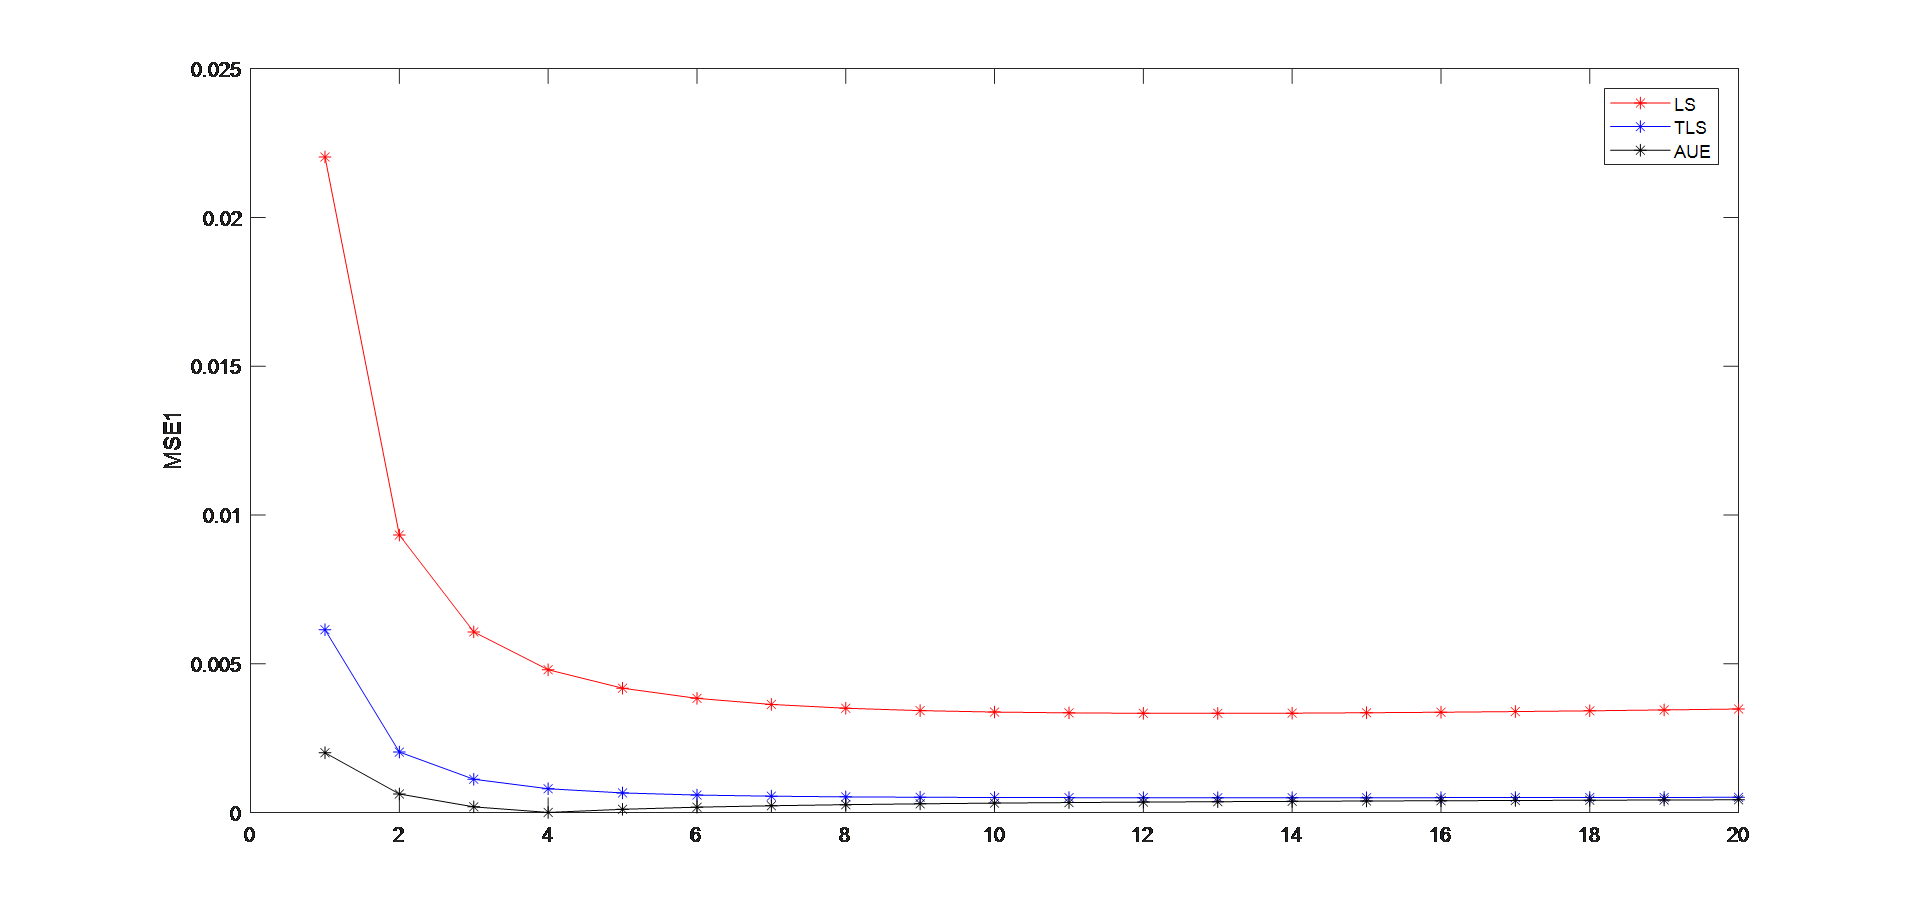
\includegraphics[width=\linewidth]{images/azimuth_MSE1.png}	
}

	\subfigure[速度相对误差图]{
	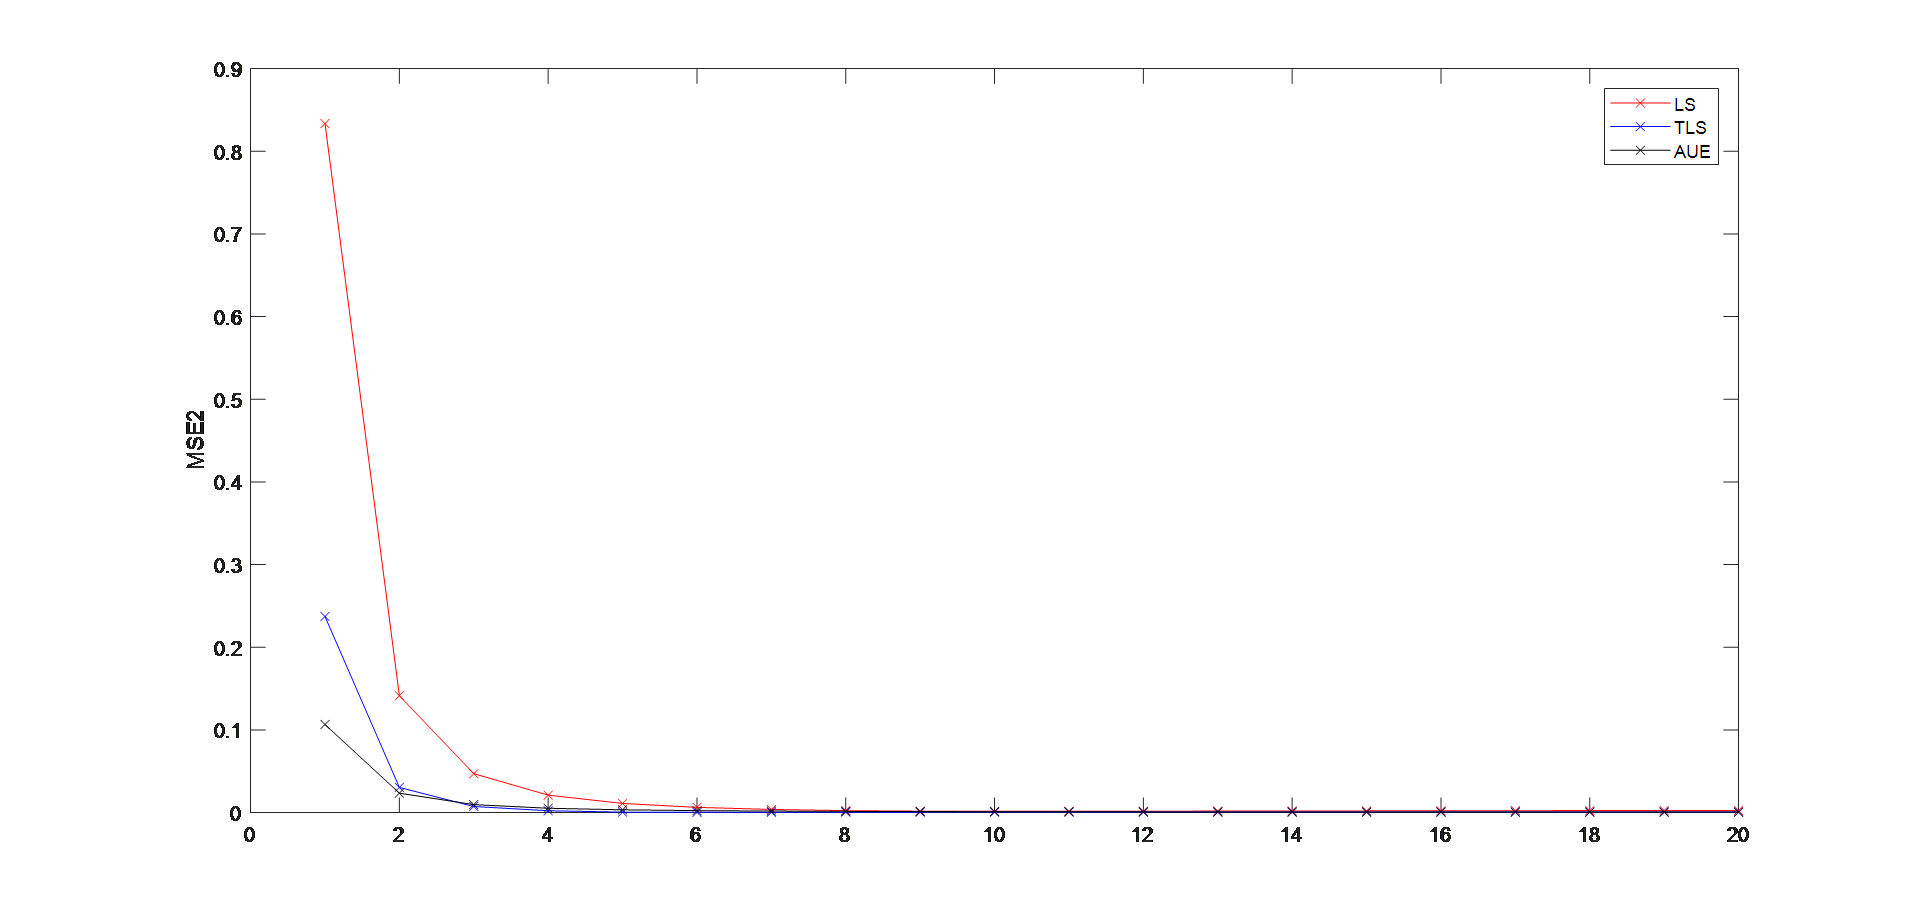
\includegraphics[width=\linewidth]{images/azimuth_MSE2.png}	
}
	\caption{方位角变化对结果的影响}
\end{figure}

从结果可以看出,当仰角间差值增大,即测量的相邻两次的仰角数据的差值变大,求解结果便会更加精确.同样的当方位角间差值增大,求解结果也会更加精确.这是因为当差值变大时,噪声对测量的结果影响变小,从而求解结果变得更加准确.
\section{测量误差对算法结果的影响}
保持观测站的运动状态不变,给定目标的速度为 $\bm{v} = (0.3km/s,0.4km/s,0.5km/s)$,在 $(x_0,y_0,z_0) \in [0,300km]\times[0,300km]\times[0,300km]$ 范围内随机选择做为初始位置,进行100次Monte Carlo实验,并分别取$\sigma=0.0005rad,\sigma=0.0001rad,\sigma=0.00005rad$,做出算法误差图.
\begin{figure}[htbp]
	\centering
	\subfigure[距离相对误差图]{
	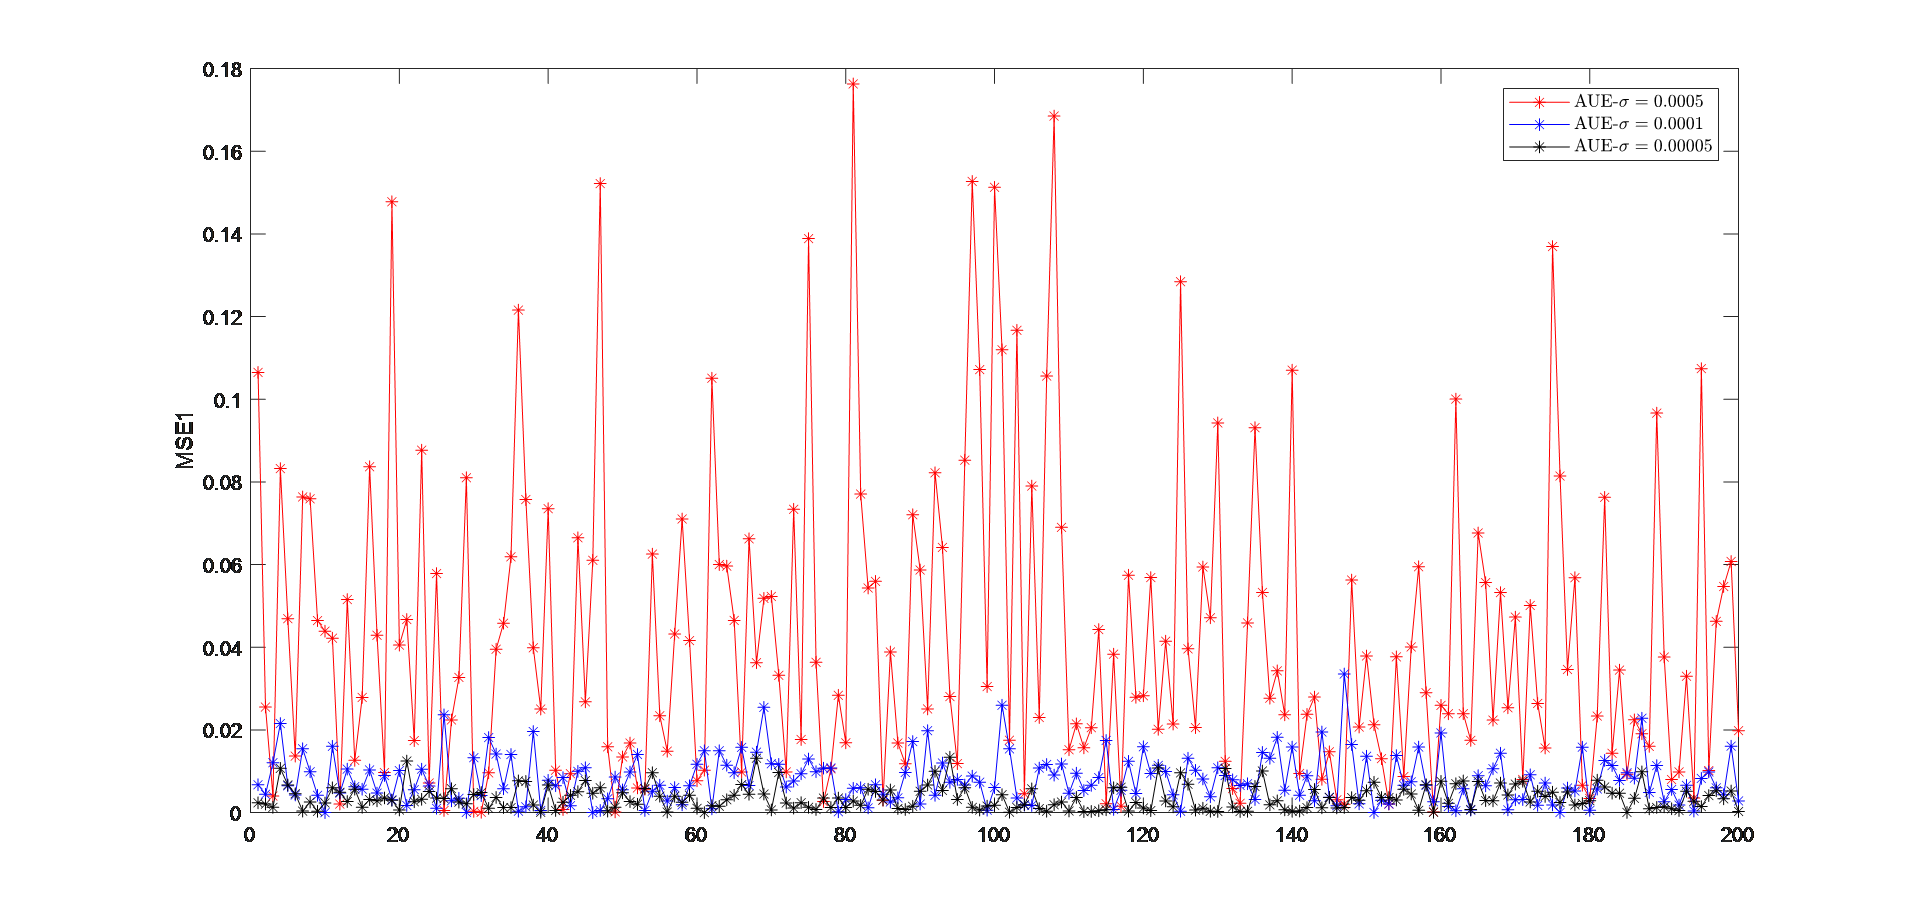
\includegraphics[width=0.93\linewidth]{images/sigma_MSE1.png}
}

	\subfigure[速度相对误差]{
	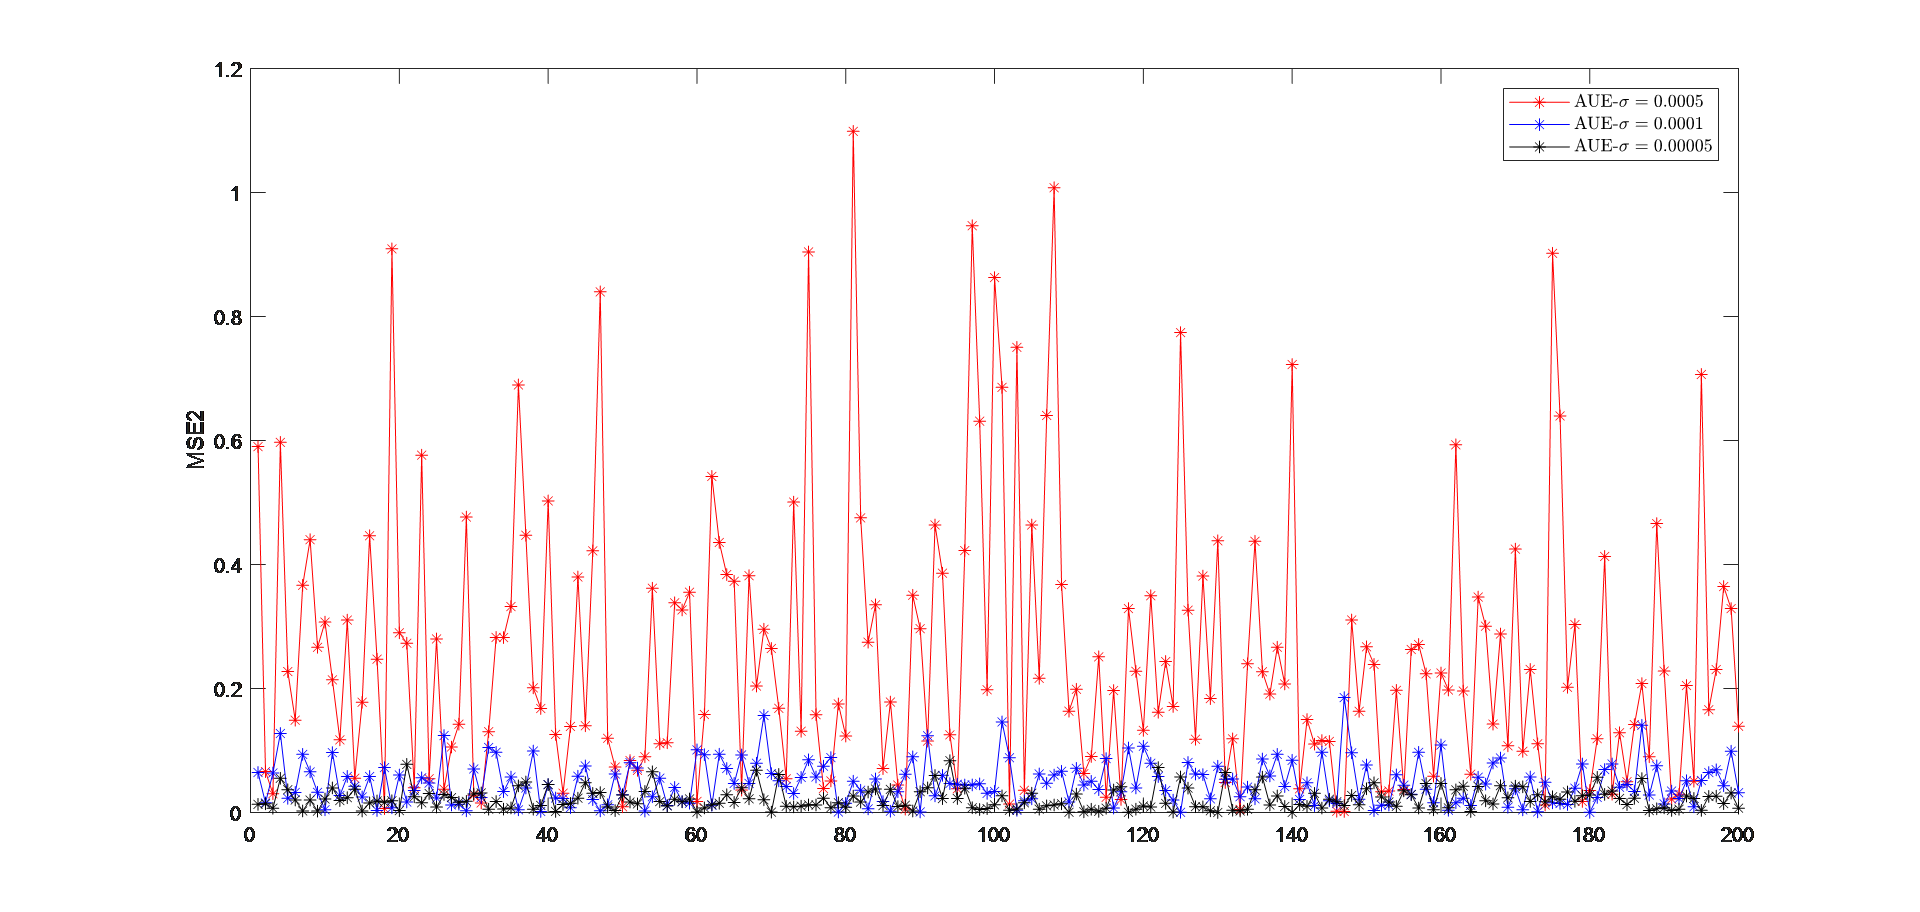
\includegraphics[width=0.93\linewidth]{images/sigma_MSE2.png}	
}
	\caption{AUE算法在不同测量误差下求解误差}
\end{figure}

由于TLS算法和AUE算法易受噪声影响,故只研究噪声对AUE算法的影响.根据上图结果可以看出,在随着测量误差的增大,AUE算法的求解结果相对误差变化幅度较大.距离相对误差的变化相对于速度相对误差的变化较小,但仍有较大误差.出现该情况的原因可能是由于目标与观测站的距离相对较大,使得真实的方位角及仰角变化不大,即实际的方位角的极差较小,仰角间的极差也相对较小,所以当噪声误差相对较大时便会对测量值产生较大的影响,使得计算得到的误差相对较大.